% NLP Lab 1 - revised, publication-style Chinese manuscript.
% Compile with XeLaTeX -> BibTeX -> XeLaTeX -> XeLaTeX.
% Place the official ACL acl.sty and acl_natbib.bst in this directory.
% Figures are vector crops from the original report.pdf, not recreated data.
\documentclass[11pt]{article}
\usepackage[preprint]{acl}
\usepackage[UTF8,scheme=plain,fontset=none]{ctex}
\usepackage{fontspec}
\IfFontExistsTF{Times New Roman}{\setmainfont{Times New Roman}}{\setmainfont{Liberation Serif}}
\IfFontExistsTF{Arial}{\setsansfont{Arial}}{\setsansfont{Liberation Sans}}
\IfFontExistsTF{Noto Serif CJK SC}{\setCJKmainfont{Noto Serif CJK SC}[AutoFakeBold=2]}{\setCJKmainfont{SimSun}[AutoFakeBold=2]}
\IfFontExistsTF{Noto Sans CJK SC}{\setCJKsansfont{Noto Sans CJK SC}[AutoFakeBold=2]}{\setCJKsansfont{Microsoft YaHei}}
\IfFontExistsTF{Noto Sans CJK SC}{\setCJKmonofont{Noto Sans CJK SC}}{\setCJKmonofont{Microsoft YaHei}}
\usepackage{amsmath,amssymb,booktabs,graphicx,array,microtype}
\usepackage{xcolor}
\usepackage{hyperref}
\definecolor{linknavy}{HTML}{25506D}
\hypersetup{colorlinks=true,linkcolor=linknavy,citecolor=linknavy,urlcolor=linknavy}
\renewcommand{\abstractname}{摘\quad 要}
\renewcommand{\refname}{参考文献}
\renewcommand{\figurename}{图}
\renewcommand{\tablename}{表}
\setlength{\emergencystretch}{1.5em}
\setlength{\textfloatsep}{12pt plus 2pt minus 2pt}
\setlength{\floatsep}{10pt plus 2pt minus 2pt}
\renewcommand{\topfraction}{0.90}
\renewcommand{\dbltopfraction}{0.90}
\renewcommand{\textfraction}{0.07}
\renewcommand{\floatpagefraction}{0.75}
\renewcommand{\dblfloatpagefraction}{0.75}
\setcounter{topnumber}{3}
\setcounter{dbltopnumber}{3}
\graphicspath{{figures/}}
\newcommand{\code}[1]{\texttt{\small #1}}
\newcommand{\macroF}{\mathrm{Macro\text{-}F1}}

\title{文本表示如何影响新闻分类：\\词袋模型、词向量与 BERT 的比较}
\author{唐健\quad 2412103\\
密码与网络空间安全学院\quad 密码科学与技术\\
自然语言处理实验一}

\begin{document}
\raggedbottom
\maketitle

\begin{abstract}
本文比较六种文本分类方法在纽约时报新闻数据集上的表现，包括二值词袋、词频词袋、在两种新闻语料上训练的 Word2Vec、预训练 GloVe 和微调 BERT。实验使用相同的训练、验证和测试划分，并同时考察准确率与宏平均 F1。二值词袋取得最高的测试准确率 99.05\% 和宏平均 F1 97.64\%；在目标数据上训练的 Word2Vec 优于外部新闻语料版本，尽管 GloVe 拥有更高的词汇覆盖率。BERT 的准确率为 98.35\%，宏平均 F1 为 96.27\%。分析发现，体育新闻容易识别，而商业与政治新闻是主要的混淆来源。BERT 仅使用文章开头的短片段，词袋与静态词向量则处理全文，这也是理解结果差异的重要条件。实验表明，对于主题清晰的长新闻，简单的词汇特征依然是一种强有力的表示。
\end{abstract}

\section{引言}

一篇新闻的主题往往可以从几个关键词中判断。球队、联赛和球员指向体育报道；公司、市场和股价通常与商业有关。然而，当一篇报道同时涉及政府政策和企业经营时，仅凭关键词就不容易区分主题。不同的文本表示方法，恰好在这两类信息之间作出了不同选择。

词袋模型保留每个词是否出现或出现多少次，因此可以直接利用主题词。Word2Vec 和 GloVe 将单词表示为低维向量，使含义相近的词获得相近表示。BERT 进一步结合上下文确定词语含义\citep{mikolov2013efficient,pennington-etal-2014-glove,devlin-etal-2019-bert}。这些方法越来越复杂，却不意味着在每一项分类任务上都能依次获得更高的准确率。简单词汇特征在文本分类中的竞争力早已有研究指出\citep{wang-manning-2012-baselines}。

本实验以 NYT 新闻三分类为例，回答三个具体问题：二值词袋和词频词袋是否存在明显差异；词向量的训练语料与词汇覆盖率如何影响分类；BERT 在输入长度受限时表现如何。除总体结果外，我们还比较各类别表现、混淆方向以及模型预测错误的文章，以解释数字背后的差异。

\section{数据与实验设置}

\subsection{数据集与划分}

NYT 数据集共有 11,519 篇有效新闻，包含商业、政治和体育三个类别。体育新闻占 75.0\%，另外两类各占约 12.5\%。这是一个明显不均衡的数据集，模型即使识别了大多数体育新闻，也可能在其他两类上表现欠佳。图~\ref{fig:distribution} 展示类别分布。

\begin{table}[t]
\centering\small
\begin{tabular}{lrrrr}
\toprule
数据集 & 商业 & 政治 & 体育 & 总计\\
\midrule
训练集 & 1,143 & 1,161 & 6,911 & 9,215\\
验证集 & 143 & 145 & 864 & 1,152\\
测试集 & 143 & 145 & 864 & 1,152\\
\midrule
全部 & 1,429 & 1,451 & 8,639 & 11,519\\
\bottomrule
\end{tabular}
\caption{NYT 新闻数据集的类别数量与划分。}
\label{tab:split}
\end{table}

\begin{figure*}[t]
\centering
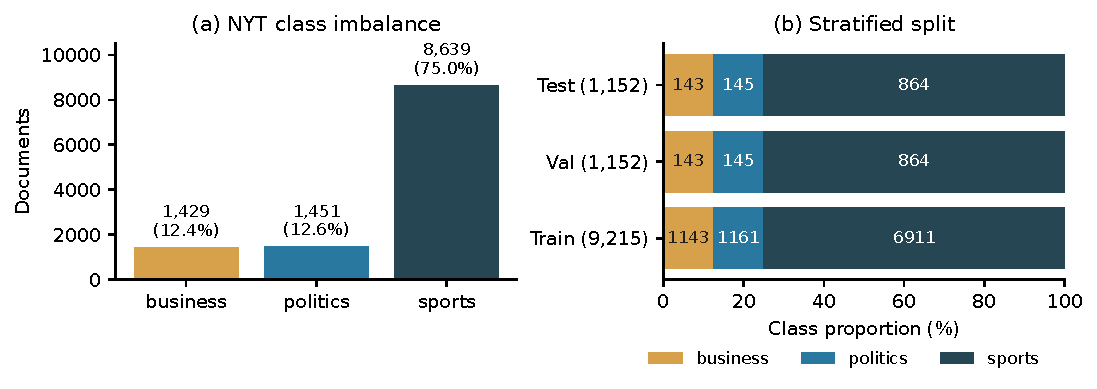
\includegraphics[width=\textwidth]{class_distribution.pdf}
\caption{NYT 数据集的类别分布。左侧为各类别样本数，右侧为训练、验证和测试集中的类别比例。}
\label{fig:distribution}
\end{figure*}

所有方法采用相同的分层随机划分。首先取 80\% 数据作为训练集，再将其余 20\% 平分为验证集和测试集，随机种子固定为 42。各集合的具体数量见表~\ref{tab:split}。另有 90,000 篇 AG News 文本，仅用于训练外部 Word2Vec，不参与 NYT 分类器的监督训练。

\subsection{评价指标}

我们使用准确率衡量整体预测的正确比例，并采用宏平均 F1（Macro-F1）衡量不同类别上的表现。对于类别 $c$，F1 由真阳性、假阳性和假阴性计算，再对三个类别取平均：
\begin{align}
\mathrm{Acc} &= \frac{1}{N}\sum_{i=1}^{N}\mathbf{1}(\hat y_i=y_i),\\
F_{1,c} &= \frac{2TP_c}{2TP_c+FP_c+FN_c},\\
\macroF &= \frac{1}{3}\sum_{c=1}^{3}F_{1,c}.
\end{align}
准确率容易受到体育这一多数类的影响，而 Macro-F1 给予三个类别相同权重。作为参照，始终预测体育类可获得 75.00\% 的准确率，但 Macro-F1 只有 28.57\%。

\subsection{训练配置}

\begin{table}[t]
\centering\small
\begin{tabular}{@{}p{.26\columnwidth}p{.66\columnwidth}@{}}
\toprule
方法 & 主要设置\\
\midrule
词袋 + LR & 60,980 维；迭代上限 2,000\\
Word2Vec & CBOW；100 维；窗口 5；最小词频 2；训练 10 轮\\
词向量 + LR & 均值池化；迭代上限 3,000\\
BERT & bert-base-uncased；最大长度 64；训练 3 轮\\
优化器 & AdamW；学习率 $2\times10^{-5}$；权重衰减 0.01\\
\bottomrule
\end{tabular}
\caption{三项任务的主要实验参数。LR 表示逻辑回归。}
\label{tab:config}
\end{table}

表~\ref{tab:config} 汇总关键配置。任务一和任务二均使用逻辑回归分类器；任务三微调整个 BERT 模型，并使用验证集 Macro-F1 选择最终模型。所有模型只在测试集上报告最终性能。

\section{三类文本表示方法}

\subsection{Task 1：词袋模型}

词袋模型将文档表示为词表上的稀疏向量。设 $n(w,d)$ 表示单词 $w$ 在文档 $d$ 中出现的次数，则二值词袋和词频词袋分别定义为
\begin{align}
x_w^{\mathrm{binary}}(d)&=\mathbf{1}[n(w,d)>0],\\
x_w^{\mathrm{freq}}(d)&=n(w,d).
\end{align}

两种表示使用相同的 CountVectorizer 和逻辑回归分类器，差别只在于是否保留词的重复次数。词表仅由训练集建立，共包含 60,980 个特征。模型可以直接为 company、government 或 football 等词学习分类权重，但无法利用词序及词语的上下文含义。

\subsection{Task 2：静态词向量}

我们比较三组 100 维词向量：在 NYT 训练集上训练的 Word2Vec、在 AG News 上训练的 Word2Vec，以及公开发布的 GloVe 6B 词向量。两组 Word2Vec 均采用 CBOW，窗口大小为 5，训练 10 轮。前两者可以比较目标语料与外部语料的差异；GloVe 则提供大规模预训练的参照\citep{mikolov2013efficient,pennington-etal-2014-glove}。

为将不同长度的新闻转换为固定维度的特征，我们对文档中的已知词向量取平均。设 $t_1,\ldots,t_m$ 是文档中能在词向量表中找到的 $m$ 个词位置，则
\begin{equation}
\mathbf z(d)=\frac{1}{m}\sum_{i=1}^{m}\mathbf e(t_i).
\label{eq:pool}
\end{equation}
同一个词出现多次就参与多次平均；未收录的词不参与计算。若没有任何词被收录，则使用零向量。最后用逻辑回归完成分类。该方法能够利用单词之间的语义联系，却会丢失词序，也无法自动突出全文中最重要的主题词。

\subsection{Task 3：BERT 微调}

任务三使用 \code{google-bert/bert-base-uncased}，在预训练编码器上增加三分类输出层，并更新所有模型参数\citep{devlin-etal-2019-bert}。训练采用 AdamW，学习率为 $2\times10^{-5}$，批次大小为 8，前 10\% 的训练步骤用于学习率预热。模型训练 3 轮，每轮结束后记录验证集结果，最终选择验证 Macro-F1 最高的检查点。

与前两项任务不同，BERT 的最大输入长度固定为 64。这个长度包含 $\mathrm{[CLS]}$ 和 $\mathrm{[SEP]}$ 等特殊标记，因此正文至多保留前 62 个 WordPiece。词袋模型与平均词向量使用全文，而 BERT 主要根据新闻开头判断类别。理解后续结果时，需要考虑这种输入范围的差别。

\section{实验结果}

\subsection{总体表现}

\begin{table*}[t]
\centering\small
\begin{tabular}{llrrrrr}
\toprule
任务 & 方法 & 验证 Acc. & 验证 Macro-F1 & 测试 Acc. & 测试 Macro-F1 & 错误数\\
\midrule
Task 1 & Binary BoW & 98.61 & 96.67 & \textbf{99.05} & \textbf{97.64} & \textbf{11}\\
Task 1 & Frequency BoW & 98.44 & 96.33 & 98.96 & 97.42 & 12\\
Task 2 & NYT Word2Vec & 97.83 & 94.99 & 98.70 & 96.72 & 15\\
Task 2 & AG Word2Vec & 96.96 & 93.37 & 98.00 & 95.17 & 23\\
Task 2 & GloVe 100d & 97.74 & 95.00 & 98.44 & 96.33 & 18\\
Task 3 & BERT 微调 & 97.57 & 94.78 & 98.35 & 96.27 & 19\\
\bottomrule
\end{tabular}
\caption{六种方法在验证集与测试集上的分类性能，单位为百分比。错误数按 1,152 篇测试新闻统计。}
\label{tab:main}
\end{table*}

\begin{figure*}[t]
\centering
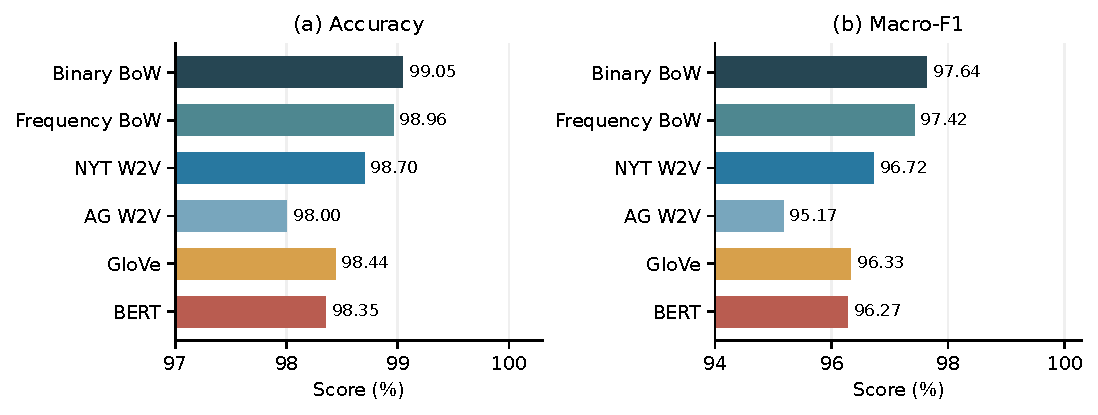
\includegraphics[width=\textwidth]{performance.pdf}
\caption{六种方法的测试准确率和 Macro-F1。为便于比较，横轴只显示分数较高的区间。}
\label{fig:performance}
\end{figure*}

表~\ref{tab:main} 和图~\ref{fig:performance} 给出了六种方法的结果。二值词袋在测试集上取得 99.05\% 的准确率和 97.64\% 的 Macro-F1，为本实验的最高值。词频词袋紧随其后，准确率为 98.96\%，Macro-F1 为 97.42\%。两者只相差一个预测正确的样本。这说明，对于当前新闻主题分类任务，词是否出现已包含大量判别信息，进一步记录出现次数并没有明显提高性能。

三种静态词向量也取得较高分数。其中 NYT Word2Vec 的 Macro-F1 为 96.72\%，GloVe 为 96.33\%，AG Word2Vec 为 95.17\%。BERT 的 Macro-F1 为 96.27\%，接近 GloVe，但低于两个词袋模型。模型规模更大、结构更复杂，并未在当前实验设置下转化为更好的分类结果。

\subsection{训练语料与词汇覆盖}

NYT Word2Vec 比 AG Word2Vec 少错 8 篇新闻，Macro-F1 高出 1.55 个百分点。虽然 AG News 有更多文章，但 NYT 训练集包含约 597 万次英文词出现，AG News 约 345 万次；两组语料在内容、篇幅和用词上也不同。NYT 词向量直接学习目标数据中的词语关系，因此可能更适合当前分类任务。

词向量能否表示测试文章中的词，也是影响效果的因素。我们分别统计词出现次数层面的未登录词比例（token OOV），以及不同词类型层面的未登录词比例（type OOV）：
\begin{align}
\mathrm{OOV}_{\mathrm{token}}&=\frac{\sum_{i=1}^{|T|}\mathbf 1[t_i\notin E]}{|T|},\\
\mathrm{OOV}_{\mathrm{type}}&=\frac{\sum_{w\in U}\mathbf 1[w\notin E]}{|U|}.
\end{align}
其中 $T$ 为测试集所有词的序列，$U$ 为其中不重复的词集合，$E$ 为词向量词表。

\begin{table}[t]
\centering\footnotesize\setlength{\tabcolsep}{2.5pt}
\begin{tabular}{@{}lrrrr@{}}
\toprule
方法 & token 数 & 占比 & type 数 & 占比\\
\midrule
NYT W2V & 5,385 & 0.71\% & 3,809 & 14.07\%\\
AG W2V & 20,082 & 2.63\% & 8,442 & 31.17\%\\
GloVe & 1,530 & 0.20\% & 807 & 2.98\%\\
\bottomrule
\end{tabular}
\caption{三种词向量在 NYT 测试集上的未登录词统计。测试集共包含 763,200 次词出现和 27,080 个不同词。}
\label{tab:oov}
\end{table}

\begin{figure*}[t]
\centering
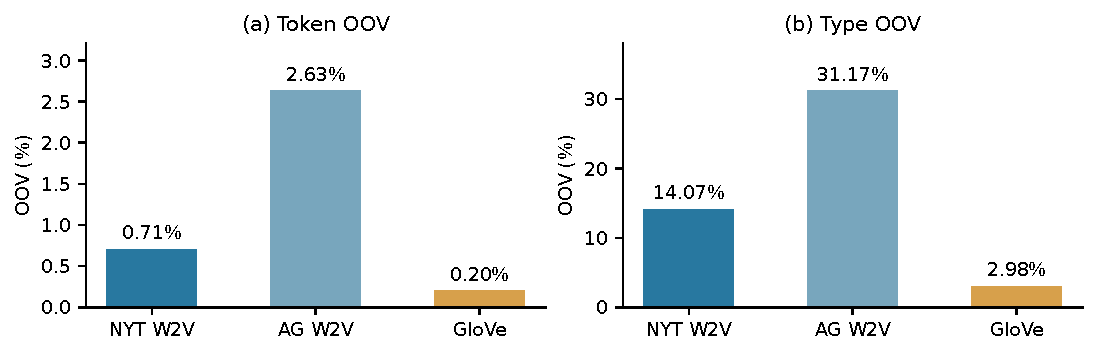
\includegraphics[width=\textwidth]{oov.pdf}
\caption{三种静态词向量的未登录词比例。GloVe 在两种统计方式下的覆盖率都是最高的。}
\label{fig:oov}
\end{figure*}

表~\ref{tab:oov} 与图~\ref{fig:oov} 呈现了一个有意思的现象。GloVe 的 token OOV 仅为 0.20\%，比 NYT Word2Vec 的 0.71\% 更低，但分类结果反而略差。较广的词汇覆盖使模型能够表示更多单词，却不保证这些表示更适合区分当前的新闻主题。训练语料与目标任务的关联，以及词向量平均后保留了多少主题信息，同样值得考虑。

\subsection{BERT 的训练过程}

\begin{figure*}[t]
\centering
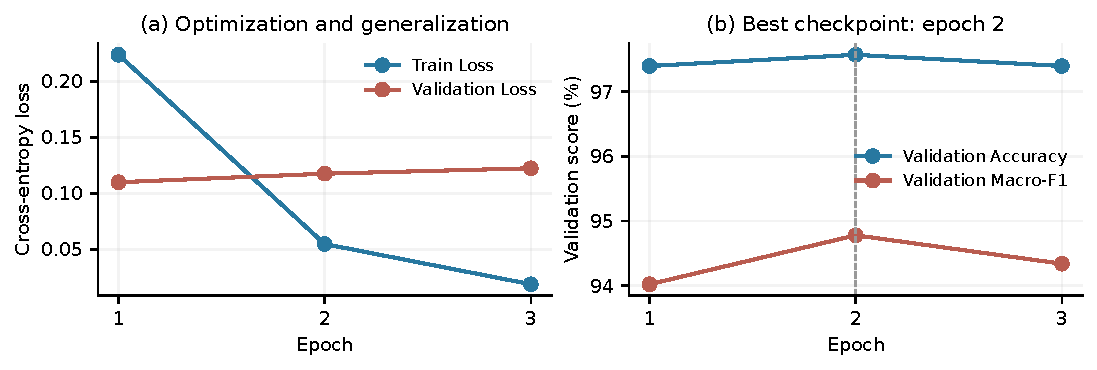
\includegraphics[width=\textwidth]{bert_training.pdf}
\caption{BERT 在三个训练轮次中的损失与验证集表现。验证 Macro-F1 在第 2 轮达到最高。}
\label{fig:training}
\end{figure*}

图~\ref{fig:training} 展示了 BERT 的训练过程。训练损失从第一轮的 0.2236 降至第三轮的 0.0188，验证损失却从 0.1098 升至 0.1223。验证 Macro-F1 分别为 94.02\%、94.78\% 和 94.34\%，第二轮达到最高，最终测试采用这一轮的模型。训练损失持续下降而验证性能没有同步提高，说明最后一轮已经出现一定的过拟合迹象。

BERT 最终准确率为 98.35\%，Macro-F1 为 96.27\%，比二值词袋分别低 0.69 和 1.37 个百分点。其输入长度只有 64 个 WordPiece 位置，而测试新闻按英文词统计的中位长度约为 697 词。两者分词单位不同，但足以看出 BERT 只能利用全文的一小部分。因此，这个结果既反映了模型表现，也受到输入长度限制，不能简单理解为上下文建模不如词袋方法。

\section{错误分析}

\subsection{类别之间的混淆}

\begin{figure*}[t]
\centering
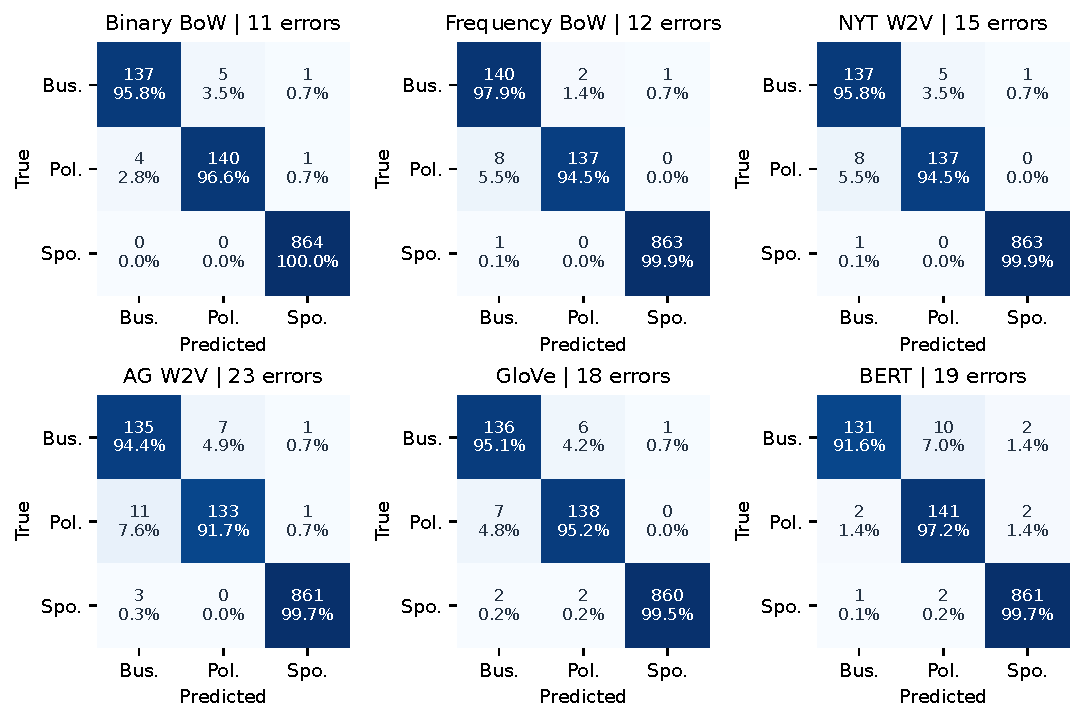
\includegraphics[width=\textwidth]{confusion_matrices.pdf}
\caption{六种方法的测试集混淆矩阵。每个单元格上方为样本数，下方为该真实类别中的比例。Bus.、Pol. 和 Spo. 分别代表商业、政治和体育。}
\label{fig:cm}
\end{figure*}

\begin{table}[t]
\centering\small\setlength{\tabcolsep}{4pt}
\begin{tabular}{lrrr}
\toprule
方法 & 商业 F1 & 政治 F1 & 体育 F1\\
\midrule
Binary BoW & 96.48 & 96.55 & 99.88\\
Frequency BoW & 95.89 & 96.48 & 99.88\\
NYT Word2Vec & 94.81 & 95.47 & 99.88\\
AG Word2Vec & 92.47 & 93.33 & 99.71\\
GloVe & 94.44 & 94.85 & 99.71\\
BERT & 94.58 & 94.63 & 99.60\\
\bottomrule
\end{tabular}
\caption{各类别在测试集上的 F1，单位为百分比。}
\label{tab:class}
\end{table}

图~\ref{fig:cm} 显示，所有方法都能非常准确地识别体育新闻，区别主要来自商业和政治类。表~\ref{tab:class} 中，体育类 F1 始终超过 99.5\%，而商业与政治类通常在 92\% 至 97\% 之间。两类新闻常同时包含政策、经济和社会议题，因此边界更容易混淆。

以 BERT 为例，143 篇商业新闻中有 10 篇被预测成政治新闻，145 篇政治新闻中则有 2 篇被预测成商业新闻。它对政治类的召回率达到 97.24\%，对商业类为 91.61\%。相比之下，NYT Word2Vec 在两个方向上的误判分别为 5 篇和 8 篇。即使最终准确率接近，两种表示也可能形成不同的决策边界。

\begin{figure*}[t]
\centering
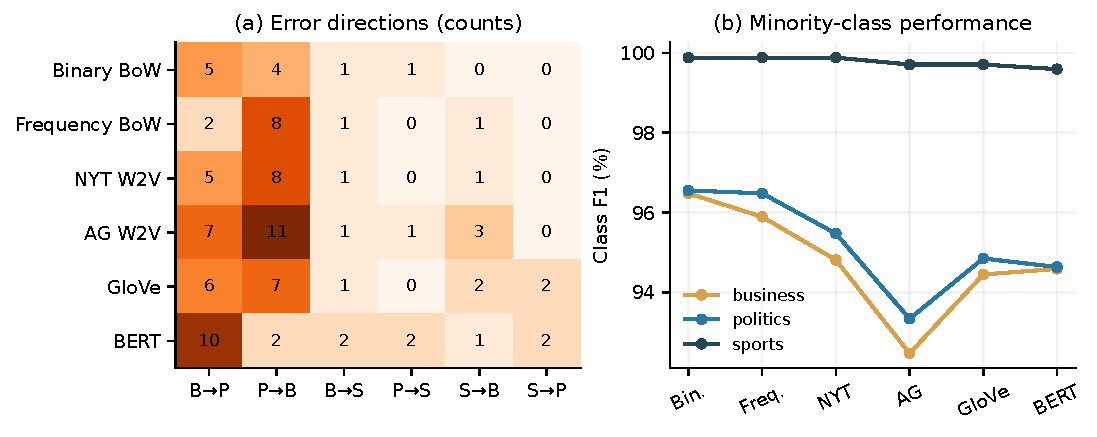
\includegraphics[width=\textwidth]{error_analysis.pdf}
\caption{六种方法的错误方向与各类别 F1。左图统计真实类别到预测类别的误判数量，右图比较各类别表现。}
\label{fig:errors}
\end{figure*}

\subsection{关键词与文档信息}

\begin{figure*}[t]
\centering
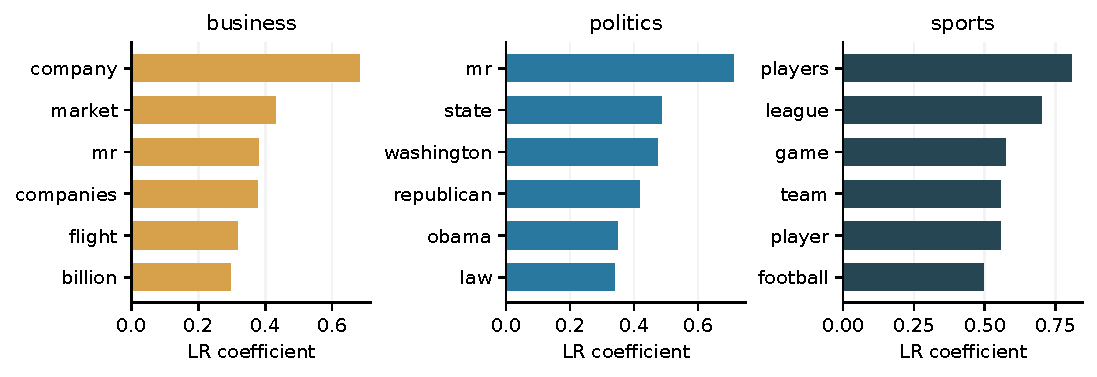
\includegraphics[width=\textwidth]{keywords.pdf}
\caption{二值词袋分类器在三个类别上权重较高的词，权重越大表示该词越有利于相应类别的判断。}
\label{fig:keywords}
\end{figure*}

图~\ref{fig:keywords} 给出了二值词袋模型的代表性特征。company、market 和 billion 与商业类相关，state、washington 和 republican 与政治类相关，players、league 和 football 则清晰地指向体育。词袋模型之所以表现出色，一个重要原因就是这些主题词可以在全文中被直接识别，并分别获得分类权重。

不过，词汇之间的联系也可能造成混淆。例如 mr 同时出现在商业和政治类的高权重词中，它更像一种新闻写作习惯，而不是明确的主题信号。与此不同，平均词向量将整篇文章压缩成一个 100 维向量，普通背景词会与主题词一起参与平均；BERT 虽能结合上下文，却只能处理文章开头的有限内容。三类方法保留的信息不同，因而会在不同新闻上犯错。

\subsection{典型错例}

\begin{table*}[t]
\centering\small
\begin{tabular}{@{}p{.12\textwidth}p{.31\textwidth}p{.31\textwidth}p{.18\textwidth}@{}}
\toprule
真实类别 $\to$ 预测类别 & 新闻内容 & 相关主题线索 & 可能的混淆原因\\
\midrule
体育 $\to$ 政治 & Ralph Wenzel 在机场跌倒，报道首先讨论其健康与照护处境。 & 后文交代他曾是一名 NFL 球员，并涉及执教经历。 & 体育背景出现较晚。\\[3pt]
政治 $\to$ 商业 & 波士顿马拉松爆炸案后，报道讨论国际学生与大学的安全问题。 & 文章涉及招生、教育选择和校园环境。 & 教育政策与学校经营主题交织。\\[3pt]
商业 $\to$ 体育 & 一篇旅行信用卡报道借 NCAA 篮球锦标赛和办公室竞猜展开叙述。 & 正文讨论 American Express、年费与机场休息室权益。 & 体育类比干扰商业主题判断。\\
\bottomrule
\end{tabular}
\caption{BERT 的三个代表性错误样本。文章内容经概括，类别与预测来自原始实验记录。}
\label{tab:cases}
\end{table*}

表~\ref{tab:cases} 中的错例展示了三种不同困难。第一篇新闻的体育身份主要出现在后文，短输入可能使模型错过关键背景。第二篇在教育、社会与政治议题之间存在交叉。第三篇一开始就谈到信用卡，却同时大量借用篮球赛事作比喻，表明即使主题词已经出现，干扰性的叙述也可能影响判断。

\begin{figure}[t]
\centering
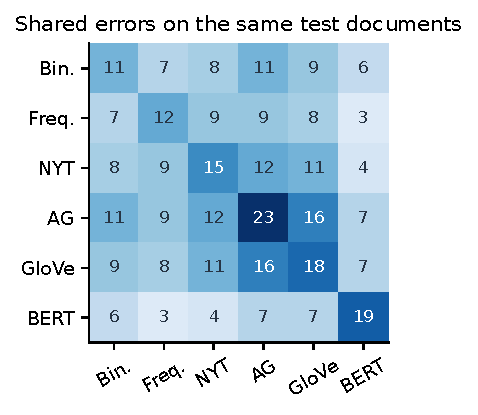
\includegraphics[width=\columnwidth]{error_overlap.pdf}
\caption{六种方法两两共同预测错误的文章数量。对角线为各方法的错误总数。}
\label{fig:overlap}
\end{figure}

图~\ref{fig:overlap} 进一步比较各方法出错的文章是否相同。二值词袋只有 11 个错例，其中与 BERT 重合的有 6 个；BERT 共错 19 篇。两种方法在部分新闻上具有互补性，也说明单看总准确率无法完整描述它们的差别。

\section{讨论}

\subsection{简单模型为何表现突出}

这组实验中，二值词袋的效果最好，首先与任务本身有关。NYT 新闻篇幅较长，类别又相对明确，全文中通常包含多次出现的主题词。词袋模型保留每个词的独立特征，让逻辑回归直接学习其类别关联；二值化还避免将同一关键词的多次出现简单等同于多倍证据。对这一任务而言，这种朴素的表示已经十分有效。

静态词向量的优势是把含义相近的词联系起来，但平均池化会削弱一些关键词的独立作用。BERT 可以捕捉更丰富的上下文，却在本实验中只能读取文章开头。三者比较的不只是模型结构，也包括不同的信息保留方式。若让全部方法处理相同长度的文本，结果可能会改变，这可以作为后续实验方向。

\subsection{实验的适用范围}

本实验使用一次固定划分，尚未通过多个随机种子检验方法排名是否稳定。此外，数据检查发现 NYT 中有 72 条重复正文记录，训练集与测试集之间有 10 篇正文完全相同。这种重叠可能使测试性能偏高。当前报告保留原始作业的划分与结果，后续若需更严格地评估泛化能力，应先按正文去重并重新训练。不同方法的分词规则和输入长度也并不完全一致，因此这里的性能对比描述的是既定实验配置，而非模型能力的绝对排序。

\section{结论}

在 NYT 新闻分类任务上，二值词袋以 99.05\% 的准确率和 97.64\% 的 Macro-F1 取得最好结果，词频词袋的表现与之接近。目标语料训练的 Word2Vec 优于外部新闻语料版本；GloVe 的词汇覆盖率最高，却没有得到最高的分类分数。BERT 的表现接近静态词向量，但受到较短输入长度的限制。

更重要的是，六种方法在体育类上都非常准确，实际差异集中在商业与政治新闻之间。实验说明，文本表示是否有效，要同时看任务中最有用的信息是什么，以及模型能够保留和利用多少这类信息。对于主题清晰的长新闻，简单的词汇表示依然具有很强的竞争力。

\bibliography{references}
\end{document}
